\documentclass{article}
\usepackage{graphicx}

% \usepackage{fancyhdr}
\usepackage[a4paper,width=180mm,top=15mm,bottom=15mm]{geometry}

% \pagestyle{fancy}
% \fancyhf{}
% \rhead{
\includegraphics[width=2cm]{uliege_logo.png}} % Replace 'example-image' with the filename of your image

\title
{
    
\includegraphics[width=5cm]{uliege_logo.png}\\[1cm]

    \textbf{MATH0001: Communication Graphique}
    \large Université de Liège - Faculté des sciences appliquées
    }

\author{Étudiant: Alexandre Detienne\\
Matricule ULiege: s2301654}

\date{20 Décembre 2023}
\begin{document}

\begin{titlepage}
    \begin{flushleft}
        
\includegraphics[width=6cm]{uliege_logo.png}
    \end{flushleft}
    \begin{center}
        \vspace{2cm}

        \LARGE{\textbf{MATH0001: Communication Graphique}}

        \vspace{0.5cm}

        \large{Université de Liège - Faculté des sciences appliquées}

        \vspace{0.5cm}

        \begin{tabular}{l l}
            Étudiant: & Alexandre Detienne\\
            \\
            Matricule: & s2301654\\
        \end{tabular}

        \vspace{2cm}

        \LARGE{\textbf{Projet-examen:} Train d'atterissage de Corsair}

        \vspace{1cm}

        Rapport
    
        \vspace{1.5cm}

        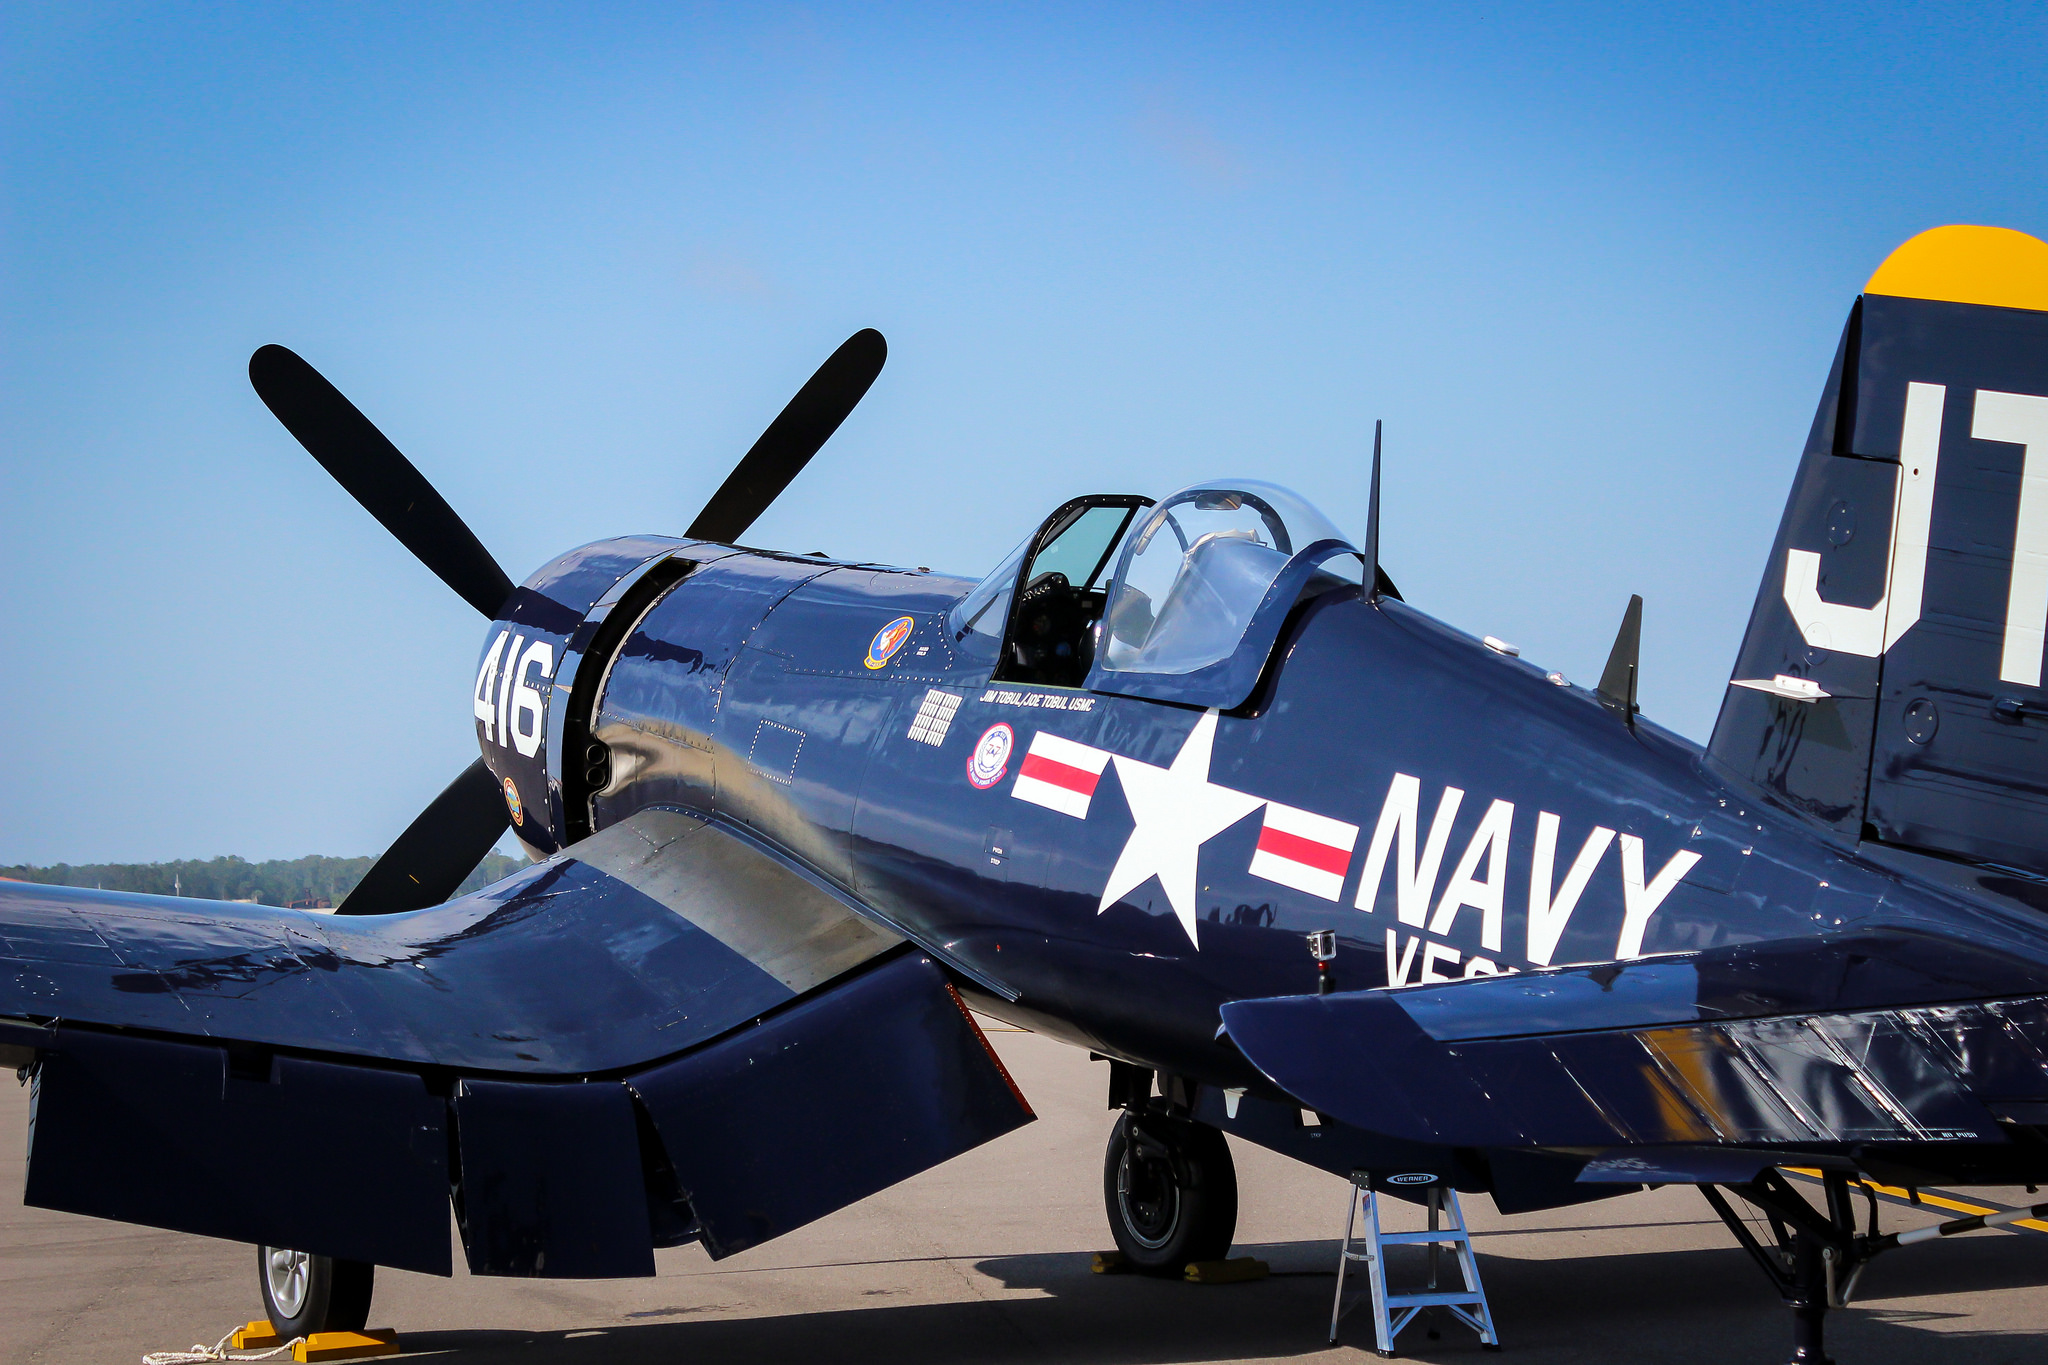
\includegraphics[width = 0.8\linewidth]{corsair_image_frontpage.jpg}

        \vspace{1cm}
    \end{center}

    \begin{flushleft}
        Année Académique 2023-2024

        NX22 - Alexandre Detienne - Décembre 2023
    \end{flushleft}
\end{titlepage}

\newpage
\tableofcontents

\newpage
\section{Données du modèle paramétrique}

Alexandre\dots

Lorem ipsum dolor sit amet, consectetur adipiscing elit, sed do eiusmod tempor incididunt ut labore et dolore magna aliqua. Duis convallis convallis tellus id interdum velit. Enim nunc faucibus a pellentesque sit amet porttitor eget dolor. Sit amet nisl purus in mollis nunc. Vitae turpis massa sed elementum tempus egestas sed sed. Amet consectetur adipiscing elit ut aliquam purus sit amet. Eget velit aliquet sagittis id consectetur. Dolor sit amet consectetur adipiscing. Sapien eget mi proin sed libero enim sed faucibus. Eget velit aliquet sagittis id consectetur purus ut.

Orci a scelerisque purus semper. Urna nunc id cursus metus aliquam eleifend mi in. Nibh venenatis cras sed felis. Scelerisque mauris pellentesque pulvinar pellentesque habitant morbi tristique senectus et. Dolor magna eget est lorem ipsum. Leo vel orci porta non pulvinar neque laoreet suspendisse. Posuere sollicitudin aliquam ultrices sagittis orci a scelerisque purus semper. Ipsum consequat nisl vel pretium lectus quam. Morbi tristique senectus et netus. Senectus et netus et malesuada fames ac turpis egestas. Dictum fusce ut placerat orci. Massa sed elementum tempus egestas sed sed risus. Sagittis eu volutpat odio facilisis mauris sit amet massa vitae.

Feugiat nibh sed pulvinar proin. At erat pellentesque adipiscing commodo elit at imperdiet dui. Pellentesque pulvinar pellentesque habitant morbi tristique senectus et netus. Vestibulum morbi blandit cursus risus. Tellus molestie nunc non blandit massa enim nec. Nullam eget felis eget nunc lobortis mattis aliquam faucibus purus. Neque ornare aenean euismod elementum nisi. A scelerisque purus semper eget. Tincidunt praesent semper feugiat nibh sed. Sit amet mattis vulputate enim nulla. Nisl vel pretium lectus quam id leo. Lorem dolor sed viverra ipsum nunc.

\section{Analyse des résultats}
\subsection{Rotation de la roue}

En faisant se déployer le train sur une durée de 20 secondes, on provoque la rotation de l'amortisseur selon son axe longitudinal, ce qui entraine une rotation de la roue.
Comme on peut le voir sur la figure~\ref{fig:wheel_rotation}, la roue aura pivoté de 88.3 degrés à la fin du mouvement d'extension du train d'atterissage, ce qui est dans les tolérances acceptées pour l'exercice.

\begin{figure}[h]
    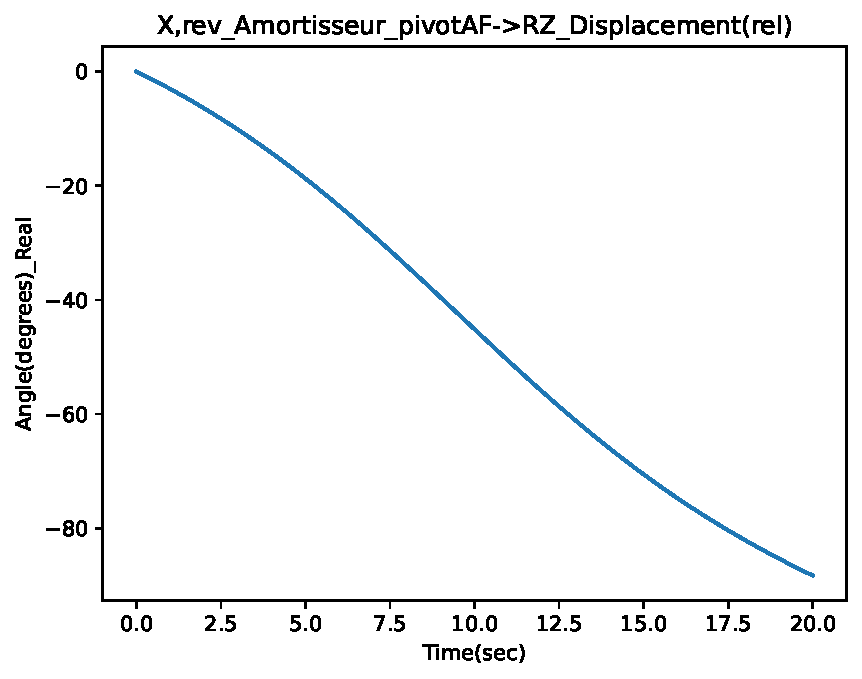
\includegraphics{data/displacement_angle_amortisseur.pdf}
    \caption{Rotation de la roue en fonction du temps}
    \label{fig:wheel_rotation}
\end{figure}
\subsection{Vitesse angulaire de l'axe principal}

La vitesse angulaire de l'axe principal...

\begin{figure}[h]
    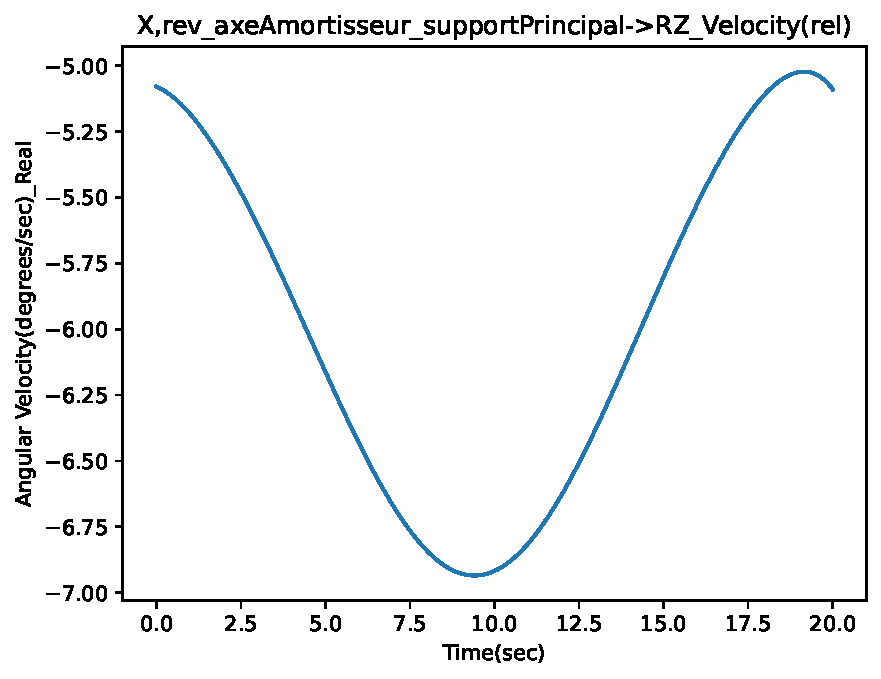
\includegraphics{data/velocity_axeAmortisseur.pdf}
    \caption{Rotation de la roue en fonction du temps}
    \label{fig:speed_main_axis}
\end{figure}

\section{Commentaires}

\end{document}